\documentclass[11pt, a4paper]{article}
\usepackage[UKenglish]{babel}
\usepackage[bibstyle=ieee, dashed=false, sorting=nty]{biblatex}
\usepackage[labelfont=bf]{caption}
\usepackage{csquotes}
\usepackage{fancyhdr}
\usepackage{float}
\usepackage{graphicx}
\usepackage[top=25mm, right=20mm, bottom=25mm, left=20mm]{geometry}
\usepackage[hidelinks]{hyperref}
\usepackage{microtype}
\usepackage{parskip}

\pagestyle{fancy}
\fancyhf{}
\fancyhead[L]{COM3504}
\fancyhead[C]{The Intelligent Web: Assignment}
\fancyhead[R]{Team: Gakki}
\fancyfoot[C]{\thepage}

\addbibresource{references.bib}

\begin{document}
\section{Introduction}
The PWA allows user to search, create, and add comments to both events and user stories. Social
features such as like, follow, interested, and going are integrated. Users are able to tag an event
with their stories, which will appear in the event page. Users can create a story by taking a
picture with their camera or upload a picture locally. Each user story can receive likes and
comments, which the latter is implemented using Socket.IO \cite{socketio, week6}. Service worker is
implemented to cache requests for offline usage. MongoDB is used to store and synchronise data
between the client and server. IndexedDB is used to store data loaded from MongoDB for offline
usage.

The Progressive Web App (PWA) allows users to search, create, tag events with stories. WebRTC is
implemented for users to take pictures with front and environment camera. Uploads are made available
for photo selection from a folder. Each story can receive likes and comments which is implemented
with SocketIO and users are able to follow one another. Attended and interested events are stored
and displayed for each user. Service worker is implemented to allow offline usage with IndexedDB
used to store data locally. MongoDB is used to store data but can only be retrieved when user is
online. The search function (via location) was implemented with Google API, allowing selected
location to be displayed on the map. For security purposes, users can only login with respective
Google Account.

\section{Diagrams}
\begin{figure}[H]
  \begin{center}
    \begin{minipage}[b]{0.4\textwidth}
      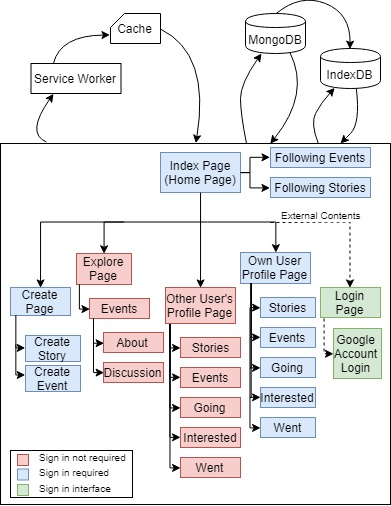
\includegraphics[width=6.8cm]{site_map.jpg}
      \caption{Demonstrates the flow of each web page in this PWA system along with the respective
      partial pages and external content pages.}
      \label{site_map}
    \end{minipage}
    %
    \qquad
    \begin{minipage}[b]{0.4\textwidth}
      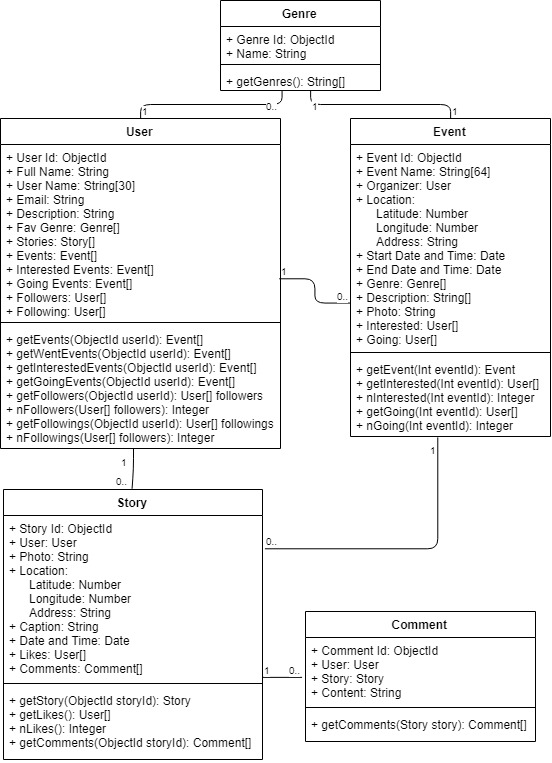
\includegraphics[width=6.8cm]{uml.jpg}
      \caption{Displays the structure of the database along with the types of content stored.}
      \label{uml}
    \end{minipage}
  \end{center}
\end{figure}
Figure~\ref{site_map} and figure~\ref{uml} are the detailed description of the PWA system structure
with figure~\ref{site_map} describing the front-end, data storage and data retrieval, while
figure~\ref{uml} describe the types of data stored in the database along with the relationship
between the documents.

\section{Interface to Insert and Search Data via Forms}
\begin{itemize}
  \item \textbf{Challenges}: 
  \begin{itemize}
    \item Usage of search libraries which would allow suggestions and auto complete. 
    \item ElasticSearch only allowed online searching and would cause errors when users are offline.
  \end{itemize}
  \item \textbf{Solution}: 
  \begin{itemize}
    \item Online library that would support offline searching so that users can make use of this 
    functionality both during online and offline
    \item Not yet implemented
  \end{itemize}
  \item \textbf{Requirements}: 
  \begin{itemize}
    \item Users should be able to search for events both during online and offline.
    \item Users should be able to search events based on events based on partial event names.
  \end{itemize}
  
  \item \textbf{Limitations}: Lorem ipsum dolor sit amet, consectetur adipiscing elit. Vivamus
  bibendum turpis in sollicitudin molestie.
\end{itemize}

\section{Interface to Search Data via Map}
\begin{itemize}
  \item \textbf{Challenges}:
  \begin{itemize}
    \item Implementation of Google API could not be cached. 
  \end{itemize}
  \item \textbf{Solution}: Not yet implemented
  \item \textbf{Requirements}: 
  \begin{itemize}
    \item Allow users to search for events' location using map.
    \item Users should be able to use this search both offline and online.
  \end{itemize}
  \item \textbf{Limitations}: Lorem ipsum dolor sit amet, consectetur adipiscing elit. Vivamus
  bibendum turpis in sollicitudin molestie.
\end{itemize}

\section{PWA – Caching of the App Template Using a Web Worker}
\begin{itemize}
  \item \textbf{Challenges}: 
  \begin{itemize}
    \item Image of events are not cached on initial load.
    \item Unable to cache user page through the use of service worker.
  \end{itemize}
  \item \textbf{Solution}: Lorem ipsum dolor sit amet, consectetur adipiscing elit. Vivamus bibendum
  turpis in sollicitudin molestie.
  \item \textbf{Requirements}: 
  \begin{itemize}
    \item Users should be able to view a basic template with required data for when offline.
    \item Users should be able to previously loaded events and stories without the ability to make any 
    changes to the events, stories, or their profiles.
  \end{itemize}
  \item \textbf{Limitations}: 
  \begin{itemize}
    \item Users are only able to view a basic offline template if no data were loaded in the past when 
    the user was online.
  \end{itemize}
\end{itemize}

\section{PWA: Caching Data Using IndexedDB}
\begin{itemize}
  \item \textbf{Challenges}:
  \begin{itemize}
    \item The usage of IndexedDB increases with every $put()$ operation. \cite{leveldb_593, leveldb_603}. 
    
  \end{itemize}
  \item \textbf{Solution}:
  \begin{itemize}
    \item There is no known solution at the moment, please refer to the links for more informat
  \end{itemize}
  \item \textbf{Requirements}:
  \begin{itemize}
    \item Optimise IndexedDB to cache data to allow offline usage with limited data available.
    \item Users should be able to access essential data when offline for the application to serve its 
    purpose.
  \end{itemize}
  \item \textbf{Limitations}: 
  \begin{itemize}
    \item IndexedDB is stored locally and could not be updated until user is online.
  \end{itemize}
\end{itemize}

\section{NodeJS Server Including Non-Blocking Organisation of Multiple Dedicated Servers}
\begin{itemize}
  \item \textbf{Challenges}: Lorem ipsum dolor sit amet, consectetur adipiscing elit. Vivamus
  bibendum turpis in sollicitudin molestie.
  \item \textbf{Solution}: Lorem ipsum dolor sit amet, consectetur adipiscing elit. Vivamus bibendum
  turpis in sollicitudin molestie.
  \item \textbf{Requirements}: Lorem ipsum dolor sit amet, consectetur adipiscing elit. Vivamus
  bibendum turpis in sollicitudin molestie.
  \item \textbf{Limitations}: Lorem ipsum dolor sit amet, consectetur adipiscing elit. Vivamus
  bibendum turpis in sollicitudin molestie.
\end{itemize}

\section{MongoDB}
\begin{itemize}
  \item \textbf{Challenges}:
  \begin{itemize}
    \item Loading of initial data to populate the database.
    \item The retrieval and storage of images in the form of bits.
  \end{itemize}
  \item \textbf{Solution}:
  \begin{itemize}
    \item Initial population of database was resolved with the use of promises.
    \item Image retrieval and storage was implemented using $base64$ encoding.
  \end{itemize}
  \item \textbf{Requirements}:
  \begin{itemize}
    \item Data stored in MongoDB is stored online. Data is not stored locally and cannot be
    retrieved offline. When user is online, data is retrieved from the database and displayed on the
    PWA.
  \end{itemize}
  \item \textbf{Limitations}:
  \begin{itemize}
    \item Initialisation of database needs to be run separately (refer to 'Extra Information').
    \item Data stored on MongoDB can only be accessed when user is online.
  \end{itemize}
\end{itemize}

\section{Quality of the Web Solution}
\begin{itemize}
  \item \textbf{Challenges}: Lorem ipsum dolor sit amet, consectetur adipiscing elit. Vivamus
  bibendum turpis in sollicitudin molestie.
  \item \textbf{Solution}: Lorem ipsum dolor sit amet, consectetur adipiscing elit. Vivamus bibendum
  turpis in sollicitudin molestie.
  \item \textbf{Requirements}: Lorem ipsum dolor sit amet, consectetur adipiscing elit. Vivamus
  bibendum turpis in sollicitudin molestie.
  \item \textbf{Limitations}: Lorem ipsum dolor sit amet, consectetur adipiscing elit. Vivamus
  bibendum turpis in sollicitudin molestie.
\end{itemize}

\section{Conclusions}
Lorem ipsum dolor sit amet, consectetur adipiscing elit. Vivamus bibendum turpis in sollicitudin
molestie.

\section{Division of Work}
Lorem ipsum dolor sit amet, consectetur adipiscing elit. Vivamus bibendum turpis in sollicitudin
molestie.

\section{Extra Information}
\begin{itemize}
  \item \textbf{Initial population of MongoDB}: run 'npm run initdb' to drop database and
  repopulate database with default data.
\end{itemize}

\printbibliography

\end{document}
